% Kommentare für den Editor (TexWorks/TexMakerX)
% !TeX encoding   = utf8
% !TeX spellcheck = de-DE

% Dokumentenklasse (Koma Script) -----------------------------------------
\documentclass[%
   %draft,     % Entwurfsstadium
   final,      % fertiges Dokument
   paper=a4, paper=portrait, pagesize=auto, % Papier Einstellungen
   fontsize=12pt, % Schriftgröße
   ngerman, % Sprache 
 ]{scrartcl} % Classes: scrartcl, scrreprt, scrbook

% ~~~~~~~~~~~~~~~~~~~~~~~~~~~~~~~~~~~~~~~~~~~~~~~~~~~~~~~~~~~~~~~~~~~~~~~~
% encoding
% ~~~~~~~~~~~~~~~~~~~~~~~~~~~~~~~~~~~~~~~~~~~~~~~~~~~~~~~~~~~~~~~~~~~~~~~~

% Encoding der Dateien (sonst funktionieren Umlaute nicht)
\usepackage[utf8]{inputenc}

% Encoding der Verzeichnisse (für Pfade mit Umlauten und Leerzeichne)
\usepackage[%
   extendedchars, encoding, multidot, space,
   filenameencoding=latin1, % Windows XP, Vista, 7
   % filenameencoding=utf8,   % Linux, OS X
]{grffile}

% ~~~~~~~~~~~~~~~~~~~~~~~~~~~~~~~~~~~~~~~~~~~~~~~~~~~~~~~~~~~~~~~~~~~~~~~~
% Pakete und Stile
% ~~~~~~~~~~~~~~~~~~~~~~~~~~~~~~~~~~~~~~~~~~~~~~~~~~~~~~~~~~~~~~~~~~~~~~~~
% Schriften
% ~~~~~~~~~~~~~~~~~~~~~~~~~~~~~~~~~~~~~~~~~~~~~~~~~~~~~~~~~~~~~~~~~~~~~~~~
% Fonts Fonts Fonts
% ~~~~~~~~~~~~~~~~~~~~~~~~~~~~~~~~~~~~~~~~~~~~~~~~~~~~~~~~~~~~~~~~~~~~~~~~

% immer laden:
\usepackage[T1]{fontenc} % T1 Schrift Encoding
\usepackage{textcomp}	 % Zusätzliche Symbole (Text Companion font extension)

% ~~~~~~~~~~~~~~~~~~~~~~~~~~~~~~~~~~~~~~~~~~~~~~~~~~~~~~~~~~~~~~~~~~~~~~~~
% Symbole
% ~~~~~~~~~~~~~~~~~~~~~~~~~~~~~~~~~~~~~~~~~~~~~~~~~~~~~~~~~~~~~~~~~~~~~~~~

\usepackage{amssymb}
\usepackage{mathcomp}


%% ==== Zusammengesetzte Schriften  (Sans + Serif) =======================

%% - Latin Modern
\usepackage{lmodern}
%% -------------------

%% - Bera Schriften
%\usepackage{bera}
%% -------------------

%% - Times, Helvetica, Courier (Word Standard...)
%\usepackage{mathptmx}
%\usepackage[scaled=.90]{helvet}
%\usepackage{courier}
%% -------------------

%% - Palantino , Helvetica, Courier
%\usepackage{mathpazo}
%\usepackage[scaled=.95]{helvet}
%\usepackage{courier}
%% -------------------

%% - Charter, Bera Sans
%\usepackage{charter}\linespread{1.05}
%\renewcommand{\sfdefault}{fvs}
%\usepackage[charter]{mathdesign}



%%%% =========== Typewriter =============

%\usepackage{courier}                   %% --- Courier
%\renewcommand{\ttdefault}{cmtl}        %% --- CmBright Typewriter Font
%\usepackage[%                          %% --- Luxi Mono (Typewriter)
%   scaled=0.9
%]{luximono}



% Pakete Laden
% ~~~~~~~~~~~~~~~~~~~~~~~~~~~~~~~~~~~~~~~~~~~~~~~~~~~~~~~~~~~~~~~~~~~~~~~~
% These packages must be loaded before all others
% (primarily because they are required by other packages)
% ~~~~~~~~~~~~~~~~~~~~~~~~~~~~~~~~~~~~~~~~~~~~~~~~~~~~~~~~~~~~~~~~~~~~~~~~
\usepackage{calc}
\usepackage{fixltx2e}	% Fix known LaTeX2e bugs

\usepackage[ngerman]{babel} 			% Sprache
\usepackage[dvipsnames, table]{xcolor} 	% Farben

% ~~~~~~~~~~~~~~~~~~~~~~~~~~~~~~~~~~~~~~~~~~~~~~~~~~~~~~~~~~~~~~~~~~~~~~~~
% Bilder, Gleitumgebungen und Platzierung
% ~~~~~~~~~~~~~~~~~~~~~~~~~~~~~~~~~~~~~~~~~~~~~~~~~~~~~~~~~~~~~~~~~~~~~~~~

\usepackage[]{graphicx}					% Graphiken
\usepackage{epstopdf}		% konvertiert eps in pdf

% provides new floats and enables H float modifier option
\usepackage{float}
% Floats immer erst nach der Referenz setzen
\usepackage{flafter}
% Alel Floats werden vor der nächsten section ausgegeben
\usepackage[section]{placeins} 
%

% ~~~~~~~~~~~~~~~~~~~~~~~~~~~~~~~~~~~~~~~~~~~~~~~~~~~~~~~~~~~~~~~~~~~~~~~~
% Beschriftungen (captions)
% ~~~~~~~~~~~~~~~~~~~~~~~~~~~~~~~~~~~~~~~~~~~~~~~~~~~~~~~~~~~~~~~~~~~~~~~~

\usepackage{caption}
\usepackage{subcaption}

% ~~~~~~~~~~~~~~~~~~~~~~~~~~~~~~~~~~~~~~~~~~~~~~~~~~~~~~~~~~~~~~~~~~~~~~~~
% Math
% ~~~~~~~~~~~~~~~~~~~~~~~~~~~~~~~~~~~~~~~~~~~~~~~~~~~~~~~~~~~~~~~~~~~~~~~~

% Base Math Package
\usepackage[fleqn]{amsmath} 
% Warnt bei Benutzung von Befehlen die mit amsmath inkompatibel sind.
\usepackage[all, error]{onlyamsmath}

% ~~~~~~~~~~~~~~~~~~~~~~~~~~~~~~~~~~~~~~~~~~~~~~~~~~~~~~~~~~~~~~~~~~~~~~~~
% Science
% ~~~~~~~~~~~~~~~~~~~~~~~~~~~~~~~~~~~~~~~~~~~~~~~~~~~~~~~~~~~~~~~~~~~~~~~~

% Einheiten und Zahlenformatierung
\usepackage{siunitx}

% ~~~~~~~~~~~~~~~~~~~~~~~~~~~~~~~~~~~~~~~~~~~~~~~~~~~~~~~~~~~~~~~~~~~~~~~~
% Tables (Tabular)
% ~~~~~~~~~~~~~~~~~~~~~~~~~~~~~~~~~~~~~~~~~~~~~~~~~~~~~~~~~~~~~~~~~~~~~~~~

\usepackage{booktabs}
\usepackage{ltxtable} % Longtable + tabularx
\usepackage{threeparttable}

% ~~~~~~~~~~~~~~~~~~~~~~~~~~~~~~~~~~~~~~~~~~~~~~~~~~~~~~~~~~~~~~~~~~~~~~~~
% text related packages
% ~~~~~~~~~~~~~~~~~~~~~~~~~~~~~~~~~~~~~~~~~~~~~~~~~~~~~~~~~~~~~~~~~~~~~~~~

\usepackage{url}            % Befehl \url{...}
\usepackage{enumitem}		% Kompakte Listen

% Neue Befehle: \Centering, \RaggedLeft, and \RaggedRight, ... 
\usepackage{ragged2e}

\usepackage{listings}
\lstset{language=bash}
\usepackage{color}

% ~~~~~~~~~~~~~~~~~~~~~~~~~~~~~~~~~~~~~~~~~~~~~~~~~~~~~~~~~~~~~~~~~~~~~~~~
% Citations
% ~~~~~~~~~~~~~~~~~~~~~~~~~~~~~~~~~~~~~~~~~~~~~~~~~~~~~~~~~~~~~~~~~~~~~~~~

%\usepackage[
%	style=alphabetic, % Loads the bibliography and the citation style 
%	natbib=true, % define natbib compatible cite commands
%]{biblatex}	
% Other options:
%	style=numeric, % 
%	style=numeric-comp,    % [1–3, 7, 8]
%	style=numeric-verb,    % [2]; [5]; [6]


% ~~~~~~~~~~~~~~~~~~~~~~~~~~~~~~~~~~~~~~~~~~~~~~~~~~~~~~~~~~~~~~~~~~~~~~~~
% layout packages
% ~~~~~~~~~~~~~~~~~~~~~~~~~~~~~~~~~~~~~~~~~~~~~~~~~~~~~~~~~~~~~~~~~~~~~~~~
%
% Befehle für 1,5 und 2 zeilig: 
% \singlespacing, \onehalfspacing und \doublespacing
\usepackage{setspace}

% ~~~~~~~~~~~~~~~~~~~~~~~~~~~~~~~~~~~~~~~~~~~~~~~~~~~~~~~~~~~~~~~~~~~~~~~~
% Kopf und Fusszeile
% ~~~~~~~~~~~~~~~~~~~~~~~~~~~~~~~~~~~~~~~~~~~~~~~~~~~~~~~~~~~~~~~~~~~~~~~~

% Kopf und Fusszeile mit scrpage2 einstellen
\usepackage[automark, komastyle, nouppercase]{scrpage2}

% ~~~~~~~~~~~~~~~~~~~~~~~~~~~~~~~~~~~~~~~~~~~~~~~~~~~~~~~~~~~~~~~~~~~~~~~~
% pdf packages
% ~~~~~~~~~~~~~~~~~~~~~~~~~~~~~~~~~~~~~~~~~~~~~~~~~~~~~~~~~~~~~~~~~~~~~~~~

% Include pages from external PDF documents in LaTeX documents
\usepackage{pdfpages} 

% Optischer Randausgleich mit pdfTeX
\usepackage{microtype}

\usepackage[unicode]{hyperref}

\usepackage{listings}
% Einstellungen und Layoutstile 
% ~~~~~~~~~~~~~~~~~~~~~~~~~~~~~~~~~~~~~~~~~~~~~~~~~~~~~~~~~~~~~~~~~~~~~~~~
% Colors
% ~~~~~~~~~~~~~~~~~~~~~~~~~~~~~~~~~~~~~~~~~~~~~~~~~~~~~~~~~~~~~~~~~~~~~~~~
\definecolor{sectioncolor}{RGB}{0, 0, 0}     % black

% ~~~~~~~~~~~~~~~~~~~~~~~~~~~~~~~~~~~~~~~~~~~~~~~~~~~~~~~~~~~~~~~~~~~~~~~~
% text related 
% ~~~~~~~~~~~~~~~~~~~~~~~~~~~~~~~~~~~~~~~~~~~~~~~~~~~~~~~~~~~~~~~~~~~~~~~~

%% style of URL
\urlstyle{tt}


% Keine hochgestellten Ziffern in der Fussnote (KOMA-Script-spezifisch):
\deffootnote{1.5em}{1em}{\makebox[1.5em][l]{\thefootnotemark}}

% Limit space of footnotes to 10 lines
\setlength{\dimen\footins}{10\baselineskip}

% prevent continuation of footnotes 
% at facing page
\interfootnotelinepenalty=10000 

% ~~~~~~~~~~~~~~~~~~~~~~~~~~~~~~~~~~~~~~~~~~~~~~~~~~~~~~~~~~~~~~~~~~~~~~~~
% Science
% ~~~~~~~~~~~~~~~~~~~~~~~~~~~~~~~~~~~~~~~~~~~~~~~~~~~~~~~~~~~~~~~~~~~~~~~~

\sisetup{%
	mode = math, detect-family, detect-weight,	
	exponent-product = \cdot,
	number-unit-separator=\text{\,},
	output-decimal-marker={,},
}

% ~~~~~~~~~~~~~~~~~~~~~~~~~~~~~~~~~~~~~~~~~~~~~~~~~~~~~~~~~~~~~~~~~~~~~~~~
% Citations / Style of Bibliography
% ~~~~~~~~~~~~~~~~~~~~~~~~~~~~~~~~~~~~~~~~~~~~~~~~~~~~~~~~~~~~~~~~~~~~~~~~

% Kommentar entfernene wenn biblatex geladen wird
% \IfPackageLoaded{biblatex}{%
	\ExecuteBibliographyOptions{%
%--- Backend --- --- ---
	backend=bibtex,  % (bibtex, bibtex8, biber)
	bibwarn=true, %
	bibencoding=ascii, % (ascii, inputenc, <encoding>)
%--- Sorting --- --- ---
	sorting=nty, % Sort by name, title, year.
	% other options: 
	% nty        Sort by name, title, year.
	% nyt        Sort by name, year, title.
	% nyvt       Sort by name, year, volume, title.
	% anyt       Sort by alphabetic label, name, year, title.
	% anyvt      Sort by alphabetic label, name, year, volume, title.
	% ynt        Sort by year, name, title.
	% ydnt       Sort by year (descending), name, title.
	% none       Do not sort at all. All entries are processed in citation order.
	% debug      Sort by entry key. This is intended for debugging only.
	%
	sortcase=true,
	sortlos=los, % (bib, los) The sorting order of the list of shorthands
	sortcites=false, % do/do not sort citations according to bib	
%--- Dates --- --- ---
	date=comp,  % (short, long, terse, comp, iso8601)
%	origdate=
%	eventdate=
%	urldate=
%	alldates=
	datezeros=true, %
	dateabbrev=true, %
%--- General Options --- --- ---
	maxnames=1,
	minnames=1,
%	maxbibnames=99,
%	maxcitenames=1,
%	autocite= % (plain, inline, footnote, superscript) 
	autopunct=true,
	language=auto,
	babel=none, % (none, hyphen, other, other*)
	block=none, % (none, space, par, nbpar, ragged)
	notetype=foot+end, % (foot+end, footonly, endonly)
	hyperref=true, % (true, false, auto)
	backref=true,
	backrefstyle=three, % (none, three, two, two+, three+, all+)
	backrefsetstyle=setonly, %
	indexing=false, % 
	% options:
	% true       Enable indexing globally.
	% false      Disable indexing globally.
	% cite       Enable indexing in citations only.
	% bib        Enable indexing in the bibliography only.
	refsection=none, % (part, chapter, section, subsection)
	refsegment=none, % (none, part, chapter, section, subsection)
	abbreviate=true, % (true, false)
	defernumbers=false, % 
	punctfont=false, % 
	arxiv=abs, % (ps, pdf, format)	
%--- Style Options --- --- ---	
% The following options are provided by the standard styles
	isbn=false,%
	url=false,%
	doi=false,%
	eprint=false,%	
	}%	
	
	% change alpha label to be without +	
	\renewcommand*{\labelalphaothers}{}
	
	% change 'In: <magazine>" to "<magazine>"
	\renewcommand*{\intitlepunct}{}
	\DefineBibliographyStrings{german}{in={}}
	
	% make names capitalized \textsc{}
	\renewcommand{\mkbibnamefirst}{\textsc}
	\renewcommand{\mkbibnamelast}{\textsc}
	
	% make volume and number look like 
	% 'Bd. 33(14): '
	\renewbibmacro*{volume+number+eid}{%
	  \setunit{\addcomma\space}%
	  \bibstring{volume}% 
	  \setunit{\addspace}%
	  \printfield{volume}%
	  \iffieldundef{number}{}{% 
	    \printtext[parens]{%
	      \printfield{number}%
	    }%
	  }%
	  \setunit{\addcomma\space}%
	  \printfield{eid}
	  %\setunit{\addcolon\space}%
	  }	

	% <authors>: <title>
	\renewcommand*{\labelnamepunct}{\addcolon\space}
	% make ': ' before pages
	\renewcommand*{\bibpagespunct}{\addcolon\space}
	% names delimiter ';' instead of ','
	%\renewcommand*{\multinamedelim}{\addsemicolon\space}

	% move date before issue
	\renewbibmacro*{journal+issuetitle}{%
	  \usebibmacro{journal}%
	  \setunit*{\addspace}%
	  \iffieldundef{series}
	    {}
	    {\newunit
	     \printfield{series}%
	     \setunit{\addspace}}%
	  %
	  \usebibmacro{issue+date}%
	  \setunit{\addcolon\space}%
	  \usebibmacro{issue}%
	  \setunit{\addspace}%
	  \usebibmacro{volume+number+eid}%
	  \newunit}

	% print all names, even if maxnames = 1
	\DeclareCiteCommand{\citeauthors}
	  {
	   \defcounter{maxnames}{1000}
	   \boolfalse{citetracker}%
	   \boolfalse{pagetracker}%
	   \usebibmacro{prenote}}
	  {\ifciteindex
	     {\indexnames{labelname}}
	     {}%
	   \printnames{labelname}}
	  {\multicitedelim}
	  {\usebibmacro{postnote}}

}%

% ~~~~~~~~~~~~~~~~~~~~~~~~~~~~~~~~~~~~~~~~~~~~~~~~~~~~~~~~~~~~~~~~~~~~~~~~
% figures, placement, floats and captions
% ~~~~~~~~~~~~~~~~~~~~~~~~~~~~~~~~~~~~~~~~~~~~~~~~~~~~~~~~~~~~~~~~~~~~~~~~

% Make float placement easier
\renewcommand{\floatpagefraction}{.75} % vorher: .5
\renewcommand{\textfraction}{.1}       % vorher: .2
\renewcommand{\topfraction}{.8}        % vorher: .7
\renewcommand{\bottomfraction}{.5}     % vorher: .3
\setcounter{topnumber}{3}        % vorher: 2
\setcounter{bottomnumber}{2}     % vorher: 1
\setcounter{totalnumber}{5}      % vorher: 3

%% ~~~ Captions ~~~~~~~~~~~~~~~~~~~~~~~~~~~~~~~~~~~~~~~~~~~~~~~~~~~~~~~~~~
% Style of captions
\DeclareCaptionStyle{captionStyleTemplateDefault}
[ % single line captions
   justification = centering
]
{ % multiline captions
% -- Formatting
   format      = plain,  % plain, hang
   indention   = 0em,    % indention of text 
   labelformat = default,% default, empty, simple, brace, parens
   labelsep    = colon,  % none, colon, period, space, quad, newline, endash
   textformat  = simple, % simple, period
% -- Justification
   justification = justified, %RaggedRight, justified, centering
   singlelinecheck = true, % false (true=ignore justification setting in single line)
% -- Fonts
   labelfont   = {small,bf},
   textfont    = {small,rm},
% valid values:
% scriptsize, footnotesize, small, normalsize, large, Large
% normalfont, ip, it, sl, sc, md, bf, rm, sf, tt
% singlespacing, onehalfspacing, doublespacing
% normalcolor, color=<...>
%
% -- Margins and further paragraph options
   margin = 10pt, %.1\textwidth,
   % width=.8\linewidth,
% -- Skips
   skip     = 10pt, % vertical space between the caption and the figure
   position = auto, % top, auto, bottom
% -- Lists
   % list=no, % suppress any entry to list of figure 
   listformat = subsimple, % empty, simple, parens, subsimple, subparens
% -- Names & Numbering
   % figurename = Abb. %
   % tablename  = Tab. %
   % listfigurename=
   % listtablename=
   % figurewithin=chapter
   % tablewithin=chapter
%-- hyperref related options
	hypcap=true, % (true, false) 
	% true=all hyperlink anchors are placed at the 
	% beginning of the (floating) environment
	%
	hypcapspace=0.5\baselineskip
}

% apply caption style
\captionsetup{
	style = captionStyleTemplateDefault % base
}

% Predefinded skip setup for different floats
\captionsetup[table]{position=top}
\captionsetup[figure]{position=bottom}


% options for subcaptions
\captionsetup[sub]{ %
	style = captionStyleTemplateDefault, % base
	skip=6pt,
	margin=5pt,
	labelformat = parens,% default, empty, simple, brace
	labelsep    = space,
	list=false,
	hypcap=false
}

% ~~~~~~~~~~~~~~~~~~~~~~~~~~~~~~~~~~~~~~~~~~~~~~~~~~~~~~~~~~~~~~~~~~~~~~~~
% layout 
% ~~~~~~~~~~~~~~~~~~~~~~~~~~~~~~~~~~~~~~~~~~~~~~~~~~~~~~~~~~~~~~~~~~~~~~~~


%% Paragraph Separation =================================
\KOMAoptions{%
   parskip=absolute, % do not change indentation according to fontsize
   parskip=false     % indentation of 1em
   % parskip=half    % parksip of 1/2 line 
}%

%% line spacing =========================================
%\onehalfspacing	% 1,5-facher Abstand
%\doublespacing		% 2-facher Abstand

%% page layout ==========================================

\raggedbottom     % Variable Seitenhoehen zulassen

% Koma Script text area layout
\KOMAoptions{%
   DIV=11,% (Size of Text Body, higher values = greater textbody)
   BCOR=5mm% (Bindekorrektur)
}%

%%% === Page Layout  Options ===
\KOMAoptions{% (most options are for package typearea)
   % twoside=true, % two side layout (alternating margins, standard in books)
   twoside=false, % single side layout 
   %
   headlines=2.1,%
}%

%\KOMAoptions{%
%      headings=noappendixprefix % chapter in appendix as in body text
%      ,headings=nochapterprefix  % no prefix at chapters
%      % ,headings=appendixprefix   % inverse of 'noappendixprefix'
%      % ,headings=chapterprefix    % inverse of 'nochapterprefix'
%      % ,headings=openany   % Chapters start at any side
%      % ,headings=openleft  % Chapters start at left side
%      ,headings=openright % Chapters start at right side      
%}%


% reloading of typearea, necessary if setting of spacing changed
\typearea[current]{last}

% ~~~~~~~~~~~~~~~~~~~~~~~~~~~~~~~~~~~~~~~~~~~~~~~~~~~~~~~~~~~~~~~~~~~~~~~~
% Titlepage
% ~~~~~~~~~~~~~~~~~~~~~~~~~~~~~~~~~~~~~~~~~~~~~~~~~~~~~~~~~~~~~~~~~~~~~~~~
\KOMAoptions{%
   % titlepage=true %
   titlepage=false %
}%

% ~~~~~~~~~~~~~~~~~~~~~~~~~~~~~~~~~~~~~~~~~~~~~~~~~~~~~~~~~~~~~~~~~~~~~~~~
% head and foot lines
% ~~~~~~~~~~~~~~~~~~~~~~~~~~~~~~~~~~~~~~~~~~~~~~~~~~~~~~~~~~~~~~~~~~~~~~~~

% \pagestyle{scrheadings} % Seite mit Headern
\pagestyle{scrplain} % Seiten ohne Header

% loescht voreingestellte Stile
\clearscrheadings
\clearscrplain
%
% Was steht wo...
% Bei headings:
%   % Oben aussen: Kapitel und Section
%   % Unten aussen: Seitenzahl
%   \ohead{\pagemark}
%   \ihead{\headmark}
%   \ofoot[\pagemark]{} % Außen unten: Seitenzahlen bei plain
% Bei Plain:
\cfoot[\pagemark]{\pagemark} % Mitte unten: Seitenzahlen bei plain


% Angezeigte Abschnitte im Header
% \automark[section]{chapter} %[rechts]{links}
\automark[subsection]{section} %[rechts]{links}

% ~~~~~~~~~~~~~~~~~~~~~~~~~~~~~~~~~~~~~~~~~~~~~~~~~~~~~~~~~~~~~~~~~~~~~~~~
% headings / page opening
% ~~~~~~~~~~~~~~~~~~~~~~~~~~~~~~~~~~~~~~~~~~~~~~~~~~~~~~~~~~~~~~~~~~~~~~~~
\setcounter{secnumdepth}{2}

\KOMAoptions{%
%%%% headings
   % headings=small  % Small Font Size, thin spacing above and below
   % headings=normal % Medium Font Size, medium spacing above and below
   headings=big % Big Font Size, large spacing above and below
}%

% Titelzeile linksbuendig, haengend
\renewcommand*{\raggedsection}{\raggedright} 

% ~~~~~~~~~~~~~~~~~~~~~~~~~~~~~~~~~~~~~~~~~~~~~~~~~~~~~~~~~~~~~~~~~~~~~~~~
% fonts of headings
% ~~~~~~~~~~~~~~~~~~~~~~~~~~~~~~~~~~~~~~~~~~~~~~~~~~~~~~~~~~~~~~~~~~~~~~~~
\setkomafont{sectioning}{\normalfont\sffamily} % \rmfamily
\setkomafont{descriptionlabel}{\itshape}
\setkomafont{pageheadfoot}{\normalfont\normalcolor\small\sffamily}
\setkomafont{pagenumber}{\normalfont\sffamily}

%%% --- Titlepage ---
%\setkomafont{subject}{}
%\setkomafont{subtitle}{}
%\setkomafont{title}{}

% ~~~~~~~~~~~~~~~~~~~~~~~~~~~~~~~~~~~~~~~~~~~~~~~~~~~~~~~~~~~~~~~~~~~~~~~~
% settings and layout of TOC, LOF, 
% ~~~~~~~~~~~~~~~~~~~~~~~~~~~~~~~~~~~~~~~~~~~~~~~~~~~~~~~~~~~~~~~~~~~~~~~~
\setcounter{tocdepth}{3} % Depth of TOC Display

% ~~~~~~~~~~~~~~~~~~~~~~~~~~~~~~~~~~~~~~~~~~~~~~~~~~~~~~~~~~~~~~~~~~~~~~~~
% Tabellen
% ~~~~~~~~~~~~~~~~~~~~~~~~~~~~~~~~~~~~~~~~~~~~~~~~~~~~~~~~~~~~~~~~~~~~~~~~

%%% -| Neue Spaltendefinitionen 'columntypes' |--
%
% Belegte Spaltentypen:
% l - links
% c - zentriert
% r - rechts
% p,m,b  - oben, mittig, unten
% X - tabularx Auto-Spalte

% um Tabellenspalten mit Flattersatz zu setzen, muss \\ vor
% (z.B.) \raggedright geschuetzt werden:
\newcommand{\PreserveBackslash}[1]{\let\temp=\\#1\let\\=\temp}

% Spalten mit Flattersatz und definierte Breite:
% m{} -> mittig
% p{} -> oben
% b{} -> unten
%
% Linksbuendig:
\newcolumntype{v}[1]{>{\PreserveBackslash\RaggedRight\hspace{0pt}}p{#1}}
\newcolumntype{M}[1]{>{\PreserveBackslash\RaggedRight\hspace{0pt}}m{#1}}
% % Rechtsbuendig :
% \newcolumntype{R}[1]{>{\PreserveBackslash\RaggedLeft\hspace{0pt}}m{#1}}
% \newcolumntype{S}[1]{>{\PreserveBackslash\RaggedLeft\hspace{0pt}}p{#1}}
% % Zentriert :
% \newcolumntype{Z}[1]{>{\PreserveBackslash\Centering\hspace{0pt}}m{#1}}
% \newcolumntype{A}[1]{>{\PreserveBackslash\Centering\hspace{0pt}}p{#1}}

\newcolumntype{Y}{>{\PreserveBackslash\RaggedLeft\hspace{0pt}}X}

%-- Einstellungen für Tabellen ----------
\providecommand\tablestyle{%
  \renewcommand{\arraystretch}{1.4} % Groessere Abstaende zwischen Zeilen
  \normalfont\normalsize            %
  \sffamily\small           % Serifenlose und kleine Schrift
  \centering%                       % Tabelle zentrieren
}

%--Einstellungen für Tabellen ----------

\colorlet{tablesubheadcolor}{gray!40}
\colorlet{tableheadcolor}{gray!25}
\colorlet{tableblackheadcolor}{black!60}
\colorlet{tablerowcolor}{gray!15.0}


% ~~~~~~~~~~~~~~~~~~~~~~~~~~~~~~~~~~~~~~~~~~~~~~~~~~~~~~~~~~~~~~~~~~~~~~~~
% pdf packages
% ~~~~~~~~~~~~~~~~~~~~~~~~~~~~~~~~~~~~~~~~~~~~~~~~~~~~~~~~~~~~~~~~~~~~~~~~

% ~~~~~~~~~~~~~~~~~~~~~~~~~~~~~~~~~~~~~~~~~~~~~~~~~~~~~~~~~~~~~~~~~~~~~~~~
% fix remaining problems
% ~~~~~~~~~~~~~~~~~~~~~~~~~~~~~~~~~~~~~~~~~~~~~~~~~~~~~~~~~~~~~~~~~~~~~~~~




% ~~~~~~~~~~~~~~~~~~~~~~~~~~~~~~~~~~~~~~~~~~~~~~~~~~~~~~~~~~~~~~~~~~~~~~~~
% Eigene Befehle
% ~~~~~~~~~~~~~~~~~~~~~~~~~~~~~~~~~~~~~~~~~~~~~~~~~~~~~~~~~~~~~~~~~~~~~~~~
% -- new commands --
\providecommand{\abs}[1]{\lvert#1\rvert}
\providecommand{\Abs}[1]{\left\lvert#1\right\rvert}
\providecommand{\norm}[1]{\left\Vert#1\right\Vert}
\providecommand{\Trace}[1]{\ensuremath{\Tr\{\,#1\,\}}} % Trace /Spur
%

\renewcommand{\d}{\partial\mspace{2mu}} % partial diff
\newcommand{\td}{\,\mathrm{d}}	% total diff

\newcommand{\Ham}{\mathcal{H}}    % Hamilton
\newcommand{\Prob}{\mathscr{P}}    % Hamilton
\newcommand{\unity}{\mathds{1}}   % Real

\renewcommand{\i}{\mathrm{i}}   % imagin�re Einheit



% -- New Operators --
\DeclareMathOperator{\rot}{rot}
\DeclareMathOperator{\grad}{grad}
\DeclareMathOperator{\Tr}{Tr}
\DeclareMathOperator{\const}{const}
\DeclareMathOperator{\e}{e} 			% exponatial Function



% ~~~~~~~~~~~~~~~~~~~~~~~~~~~~~~~~~~~~~~~~~~~~~~~~~~~~~~~~~~~~~~~~~~~~~~~~
% Eigene Befehle
% ~~~~~~~~~~~~~~~~~~~~~~~~~~~~~~~~~~~~~~~~~~~~~~~~~~~~~~~~~~~~~~~~~~~~~~~~
% Silbentrennung hinzufügen als 
% Sil-ben-tren-nung 
\hyphenation{}

\listfiles % schreibt alle verwendeten Dateien in die log Datei

%% Dokument Beginn %%%%%%%%%%%%%%%%%%%%%%%%%%%%%%%%%%%%%%%%%%%%%%%%%%%%%%%%
\begin{document}

% Automatische Titelseite


% Manuelle Titelseite

\begin{titlepage}
   \mbox{}\vspace{5\baselineskip}\\
   \sffamily\huge
   \centering
   % Titel
   {\Huge Projektbericht} \\
   \normalsize Modeler 2018
   \vspace{3\baselineskip}\\
   \rmfamily\Large
  Fachhochschule Bielefeld \\
  Campus Minden \\
  Studiengang Informatik
   \vspace{1\baselineskip}\\
\noindent\rule{15cm}{0.3pt}
Beteiligte Personen:
\begin{table}[H]
	\tablestyle
	\rowcolors{1}{tablerowcolor}{white!100}
	\begin{tabular}{*{2}{v{0.45\textwidth}}}
		\hline
		\rowcolor{tableheadcolor}
		\textbf{Name} &
		\textbf{Matrikelnummer} \tabularnewline
		\hline
		Johannes Ens & 1047037\tabularnewline
		Daniel Sprick & 0000000\tabularnewline
		Martin Ziel & 1078228\tabularnewline
		Eduard Ljaschenko& 1027656\tabularnewline

	\end{tabular}
\end{table}
   \noindent\rule{15cm}{0.4pt}

   \today
\end{titlepage}



\tableofcontents

% Testdokumente (auskommentieren!)
% \newcommand{\env}[1]{\texttt{#1}}
\newcommand{\command}[1]{\texttt{#1}}
\newcommand{\package}[1]{\texttt{\itshape#1}}
\newcommand{\engl}[1]{(engl: \textit{#1})\xspace}
\newpage

\section*{\LARGE Hinweis zur Erstellung von Praktikumsprotokollen} 
Die Erstellung von Praktikumsprotokollen dient der Vorbereitung sowohl auf die akademische als auch auf die praktische Arbeit. Daher sind die gängigen Regeln des wissenschaftlichen Arbeits einzuhalten. Im Protokoll soll jede Phase des Versuchs bzw. des Praktikums festgehalten und entsprechend dokumentiert werden. Im Folgenden werden die wichtigen Teilaspekte dargestellt und besprochen.

\subsection*{Deckblatt}

Verwenden Sie am Besten, dass bereits vorbereitete Deckblatt. Sollten Sie ein eigenens Deckblatt bevorzugen, sind mindestens die folgenden Einträge zu übernehmen:

\begin{itemize}
	\item Praktikumstitel und Praktikumsnummer
	\item Datum
	\item Versuchsteilnehmer mit Matrikelnummer
	\item Protokollführer (Erste Stelle der Versuchsteilnehmer)
\end{itemize}

\subsection*{Frage- bzw. Aufgabenstellung}
Für jede Teilaufgabe ist die bearbeitete Frage- bzw. Aufgabenstellung unbedingt mit zu übertragen. (Nicht nur die Nummer !)

\subsubsection{Lösungsweg}
Beschreiben Sie die Durchführung der Aufgabenstellung. Hieraus folgt, dass Sie nicht nur die Ergebnisse festhalten, sondern auch den Weg dahin und zwar so kleinschrittig wie nötig und \underline{sinnvoll}. Aufgetretene Effekte bzw. Probleme sind ebenso festzuhalten. Ziel ist es den Versuch für Dritte nachvollziehbar zu gestalten.

\subsubsection{Ergebnisse}
Beschreiben Sie in jedem Fall die erzielten Ergebnisse. Selbst wenn ein Versuch nicht das gewünschte Ergebnis erziehlt hat, sollten Sie diese trotzdem dokumentieren. (Nicht dokumentierte Ergebnisse können keine Punkte erreichen)

\subsubsection{Diskussion}
\begin{itemize}
	\item In jedem Fall sollte innerhalb der Diskussion auf die Fragestellung eingegangen werden, jedoch sind auch weitere Aspekte des Versuchs zu diskutieren.
	\newpage
	\item Probleme und besondere Vorkomnisse: Probleme können auftreteten, sollten jedoch in jedem Fall im Protokoll festgehalten werden. Neben der Meldung bei dem entsprechenden Betreuer sind folgende Punkte zu dokumentieren:
	\begin{itemize}
		\item was aufgetreten ist und unter welchen Bedingungen
		\item was Sie versucht haben und mit welchen Ergebnissen
		\item die möglichen Ursachen des Problems
	\end{itemize}
\end{itemize}

\subsubsection{Rückmeldung}
Wir würden uns freuen, wenn Sie das Protokoll auch durchaus nutzen, um Rückmeldung zu den Praktikas zu geben. Gab es Probleme bei der Hardware, ist die Organisation verbesserungswürdig oder gab es unklare Fragestellungen. \\

\textbf{Hinweis}: Sollten wir den Eindruck erlangen, dass Sie das Protokoll nicht eigenständig (in Ihrer Gruppe) angefertigt haben oder dass das Protokoll auf Basis von den Ergebnissen anderer Gruppen angefertigt wurde, wird das entsprechende Praktikum mit 5.0 bewertet und die Abgabe als Täuschungsversuch gesehen.
\\

\textbf{Hinweis:} Neben der Abgabe des Protokolls ist die Teilnahme an Praktikas weiterhin Pflicht und eine notwendige Teilleistung für das Bestehen des Praktikums. In diesen werden Sie Ihre Ergebnisse vorstellen und wir werden diese besprechen.
% \input{content/demo/demo.tex}
% \input{content/demo/latexexample.tex}

% in diese Datei gehört der Inhalt des Dokumentes:
\newpage
	\section{\Large EINLEITUNG}
	Die in diesem Dokument beschriebene Software, ist eine Modeler-Software, die dazu imstande ist Körper und Flächen zu erstellen. Außerdem lassen sich die erstellten Modelle als OBJ-Datei speichern. Gespeicherte Modelle können geladen und auch bearbeitet werden.\newline
Zur Erstellung der Software wurde die Programmiersprache C/C++ genutzt unter Verwendung von OpenGL und ist mit Linux als auch mit Windows kompatibel.
	
	
	\section{\Large BEDIENUNG}
	\begin{labeling}[]{\textbf{Gewichtung der ausgewählte Punkte:}}%längster Wert 
		\item [\textbf{OBJ-Datei laden:}] \textbf{File} $\rightarrow$ \textbf{Open} oder \textbf{Strg + O}
		\item [\textbf{Neues Objekt:}] \textbf{File} $\rightarrow$ \textbf{New} oder \textbf{Strg + N}
hh		\item [\textbf{Objekt als OBJ speichern:}] \textbf{File} $\rightarrow$ \textbf{Save} oder \textbf{Strg + S}
		\newline
		\item [\textbf{Kamera Position verändern:}] '\textbf{w}',  '\textbf{a}', '\textbf{s}', '\textbf{d}', '\textbf{q}', '\textbf{e}' - Tasten
		\item [\textbf{Kameraausrichtung ändern:}] \textbf{linke Maustaste} + bewegen der Maus
		\newline
		\item [\textbf{Raster de/aktivieren:}] '\textbf{g}' - Taste
		\item [\textbf{Punkte de/aktivieren:}] '\textbf{p}' - Taste
		\item [\textbf{Kanten de/aktivieren:}] '\textbf{k}' - Taste
		\newline
		\item [\textbf{Punkt/e auswählen:}] \textbf{Strg} + Klick auf Punkt
		\item [\textbf{Neuer Punkt:}] \textbf{rechte Maustaste} auf Raster oder Objekt
		\item [\textbf{Ausgewählte Punkte löschen:}] '\textbf{r}' - Taste
		\item [\textbf{Ausgewählte Punkte verschieben:}] Pfeiltasten, '\textbf{+}' und  '\textbf{-}'
		\newline
		\item [\textbf{Erstellung eines Face:}] Punkte gegen Uhrzeigersinn auswählen +  '\textbf{f}' - Taste
		\newline
		\item [\textbf{Catmull-Clark Unterteilung:}]  '\textbf{c}' - Taste je Schritt
		\item [\textbf{Unterteilung zurücksetzen:}] '\textbf{Strg + Z}
		\newline
		\item [\textbf{Gewichtung der ausgewählte Punkte:}] \textbf{Vertex} $\rightarrow$ \textbf{VertexWeight}
		\newline
		\item [\textbf{Smoothing:}]  '\textbf{l}' - Taste je Schritt
	\end{labeling}
		
	\section{\Large SHADER}
	Das Programm verwedet einen \textbf{Vertex Shader} und einen \textbf{Fragment Shader} für die Umsetzung des \textbf{Goroud shadings}. In die Beleuchtungs-Berechnung fließen die Position der Primären Lichtquelle, die Farbe dieser Lichtquelle sowie weitere Faktoren wie die Farbe und Stärke des Umgebungslichtes und die Eigenschaften des Materials hinsichtlich der Spiegelungen. In Abhängigkeit des Betrachtungswinkels wird die Beleuchtung berechnet indem die Normalen an den Vertices interpoliert werden. Außerdem werden mithilfe der Shader die Vertices als Kreise dargestellt.\newline\newline
 	Vorhergegangene Versuche zeigten deutlich, dass die Darstellung der Vertex-Punkte nicht effizient gelöst werden kann wenn jeder Punkt durch ein eigenes VAO repräsentiert wird. Im Zuge dieser Erkenntnis entschloss sich das Team die Punkte darzustellen indem alle Vertices mithilfe des Parameters GL\_POINTS als Point-Cloud gerendert werden. Diese Lösung ist effizient, jedoch ergab sich das Problem, dass die Punkte mit GL\_POINTS als Vierecke gerendert wurden. Die Lösung für dieses Problem besteht darin einen Radius zu definieren und alle Fragmente, die sich Außerhalb dieses Radius befinden, nicht zu rendern. Da die Größe dieser Kreise nicht in Raumkoordinatengrößen definiert werden, sondern in Pixelgröße, wurden die Punkte alle gleich groß, unabhängig von der Entfernung, gerendert. Um eine Dynamische Größe zu gewährleisten, wird die Entfernung der Kamera zu dem Punkt berechnet und der Radius des Punktes wird proportional zur Entfernung kleiner.
	
	\section{\Large KAMERA}
	Um das Betrachten des Objektes von allen Seiten zu ermöglichen endschied sich das Team eine Lösung zu implementieren die \textbf{Quaternionen} nutzt. So wurde eine Computerspiel-artige Steuerung der Kamera entwickelt, welche es ermöglicht die Ausrichtung der Kamera mithilfe der Maus zu beeinflussen und die Position der Kamera mithilfe der Tasten w, a, s, d, q und e zu verändern. Beim Drücken der Linken Maustaste und ziehen in eine Richtung wird eine Achse definiert, welche senkrecht zu der gezogenen Bahn steht. Um diese Achse wird die Ausrichtung der Kamera während der Bewegung rotiert.
		
	\section{\Large ARCHITEKTUR}
	
	\begin{figure}[H]
	\centering
	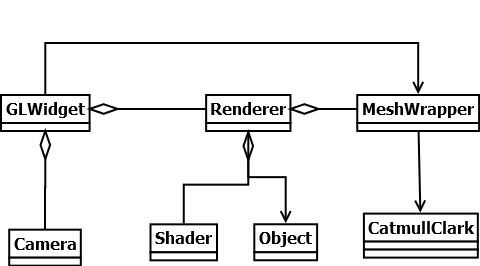
\includegraphics[width=0.7\linewidth]{uebersicht.png}
	\caption{Übersicht}
	\label{fig1}
	\end{figure}

	\begin{figure}[H]
	\centering
	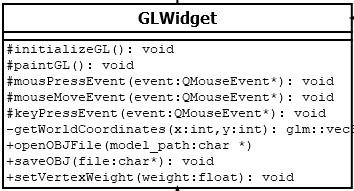
\includegraphics[width=0.7\linewidth]{GLWidget.png}
	\caption{GLWidget}
	\label{fig2}
	\end{figure}
	
	Die Klasse \textbf{GLWidget} erweitert die QT-Klasee \textbf{QGLWidget} und und gibt Funktionen wie das Laden einer OBJ-Datei oder das Speichern einer OBJ-Datei, sowie das setzen der Vertex-Gewichtung an den MeshWrapper weiter.\newline\newline

	\begin{labeling}[]{[\textbf{getWorldCoodinates()}}%längster Wert 
	\item[\textbf{initializeGL()}] OpenGL Funktionalitäten werden initialisiert, Kamera wird konfiguriert und Renderer wird mit seinem Shader-Programm geladen.
	\item[\textbf{paintGL()}] Diese Funktion wird von QT in einer Rendering-Schleife aufgerufen, aktualisiert die Attribute der Kamera und bindet  die aktuellen Matrizen, die von dem Shader benötigt werden, an den Shader.
	\item[\textbf{mousePressEvent()}] Durch das Drücken einer Maustaste ausgelöst, führt die Aktionen \textbf{Vertex-Auswahl} und \textbf{Vertex-Erzeugung} aus. Beide Aktionen bedienen sich der Funktion \textbf{getWorldCoordinates()}.
	\item[\textbf{getWorldCoodinates()}]  implementiert Ray-Picking verfahren mithilfe der Funktionen \textbf{gluUnProject()} und \textbf{glReadPixels()}. In dem Ray-Picking Verfahren wird ein Strahl durch die 3D-Welt zwischen Near- und Far-Pane projiziert. Die Koordinaten im 3D-Raum an denen zuerst ein gerendertes Objekt gekreuzt wird, werden als Rückgabewert der Funktion \textbf{getWorldCoordinates()} zurück geliefert. Aus diesem Grund bestand die Notwendigkeit eine Fläche in der 3D-Welt zu rendern die von einem Raster überlagert wird. Diese Fläche ermöglicht es Vertices per Mausklick mittels des Ray-Picking Verfahren hinzuzufügen. Die Fläche inklusive dem Raster können ausgeblendet werden, wenn sie beispielsweise beim Betrachten oder bearbeiten eines Objektes stören.
	\item[\textbf{keyPressEvent()}] behandelt weitere Benutzerinteraktionen wie die Bewegung durch den Raum oder die Manipulation des Mesh und gibt diese an die jeweiligen Klassen weiter.
	\end{labeling}
		
	\begin{figure}[H]
	\centering
	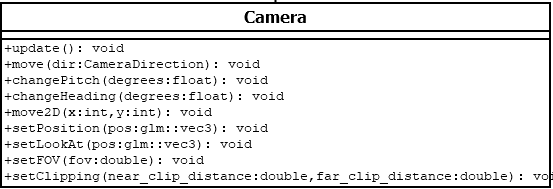
\includegraphics[width=0.7\linewidth]{camera.png}
	\caption{Camera}
	\label{fig3}
	\end{figure}

Kamera Text ...

	\begin{figure}[H]
	\centering
	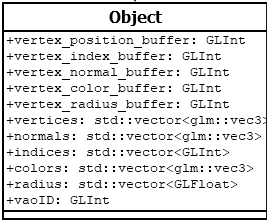
\includegraphics[width=0.7\linewidth]{object.png}
	\caption{Object}
	\label{fig4}
	\end{figure}

\noindent Die Klasse \textbf{Object} wird im Renderer benötigt. Hier werden alle Daten zu einem Objekt, welches gerendert werden soll, gespeichert. Die Daten bestehen aus den ID´s der unterschiedlichen Buffer-Objects, der ID des Vertex-Array-Objektes, sowie den Daten die dieses Objekt definieren. Der Renderer ist so Implementiert das nicht zwangsläufig alle Attribute des Objekts definiert sein müssen. Beispielsweise wird davon ausgegangen, dass die Vertices in Triangulierter-Form und Reihenfolge im vertex\_position\_buffer vorliegen, wenn der vertex\_index\_buffer nicht definiert ist.

	\begin{figure}[H]
	\centering
	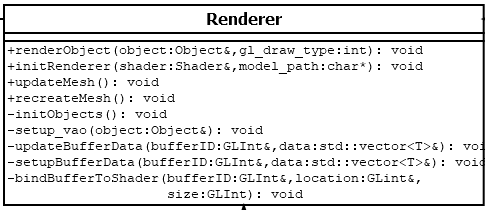
\includegraphics[width=0.7\linewidth]{renderer.png}
	\caption{Renderer}
	\label{fig5}
	\end{figure}

	\noindent In dieser Klasse werden alle Operationen ausgeführt die den Rendering-Prozess betreffen. Die Klasse hält verschieden Instanzen der Object Struktur. Das Mesh wird in dreifacher Variation als Object gehalten:
	\begin{enumerate}
	\item für die Darstellung der Flächen
	\item für die Darstellung der Punkte
	\item für die Darstellung der Linien, die die Kanten der Faces visualisieren.
	\end{enumerate}
Außerdem werden Objects für das Raster sowie die Fläche unterhalb des Rasters initialisiert.\newline
Bei der Initialisierung der einzelnen Objekte werden die Daten-Attribute der Object Instanz belegt und für jedes Objekt wird ein VAO erstellt sowie die buffer\_objects der Daten-Attribute, die belegt sind, werden erzeugt. Hierfür werden die Template-Funktion \textbf{setup\_buffer\_data()} und \textbf{bindBufferToShader()} verwendet. \textbf{updateBufferData()} ist eine Template-Funktion, welche \textbf{glBufferSubData} nutzt um die gespeicherten Daten zu aktualisieren. Dies geschieht zum Beispiel, wenn ein Vertex-Punkt verschoben wird. Wird ein Punkt hinzugefügt, entfernt oder ein Face erstellt, wird die Größe des Buffer-Objects verändert. Für diesen Fall eignet sich \textbf{glBufferSubData} nicht mehr und die entsprechende Buffer-Objects werden mittels \textbf{recreateMesh()} neu erstellt.\newline
Bei der Initialisierung der Renderer Instanz werden die Dimensionen des Mesh-Objektes berücksichtigt. Es werden die Minimalen und Maximalen Vertex-Positionen ermittelt und das Raster-Objekt wird unterhalb der niedrigsten Position auf der Y-Achse positioniert. Zusätzlich wird das Raster auf eine Größe, die 50\% größer als die Differenz aus der Maximalen X und Minimalen X Position oder, wenn diese größer ist, die Differenz auf der Z-Achse, beschränkt.

	\begin{figure}[H]
	\centering
	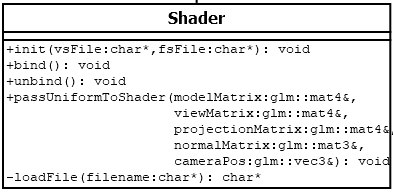
\includegraphics[width=0.7\linewidth]{shader.png}
	\caption{Shader}
	\label{fig6}
	\end{figure}

\noindent Die Shader-Klasse bindet die übergebenen zwei GLSL-Shader an die Grafikkarte. Hierfür werden die übergebenen Shader ausgelesen und die benötigten Parameter an die Shader weitergeleitet. In unserem Programm beschränken wir uns auf die Verwendung eines \textbf{Vertex-Shaders} und eines \textbf{Fragment-Shaders}, welche das \textbf{Gouroud-Shading} umsetzen und für die korrekte Darstellung der Punkte zuständig sind.

	\begin{figure}[H]
	\centering
	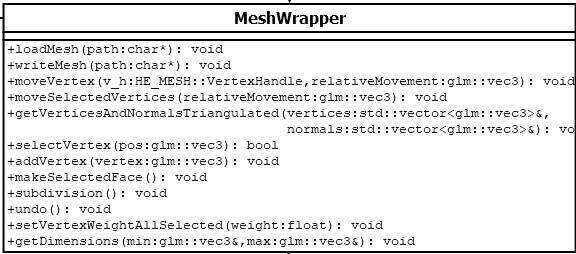
\includegraphics[width=0.7\linewidth]{meshWrapper.png}
	\caption{Meshwrapper}
	\label{fig7}
	\end{figure}

\noindent Der \textbf{MeshWrapper} schachtelt die OpenMesh-Funktionalitäten und schafft eine Schnittstelle um die Interaktion mit dem Mesh zu ermöglichen. Für die Konfiguration des Meshes wird ein struct verwendet welches festlegt, dass die Punkte und Normalen als float gespeichert werden. Somit ist die Integration in die Umgebung, welche vorwiegend mit dem Datentyp float arbeitet gewährleistet. Da für die Gewichtung der Vertices bei der Berechnung der Unterteilungsflächen eine vierte Komponente benötigt wird, wird die Klasse \textbf{HE\_MESH} genutzt, welche von der Klasse PolyMesh, aus der OpenMesh-Bibliothek, abgeleitet wird.\newline
Der MeshWrapper verfügt über ein Objekt der Klasse \textbf{HE\_MESH}. Dieses Objekt repräsentiert das Mesh. Außerdem wird ein std::vector verwendet der die aktuell markierten Vertices speichert. Zudem wird ein Backstack angelegt, der bei jeder Ausführung des Catmull-Clark Unterteilungsflächen-Algorithmus, das Mesh speichert. Dadurch kann jeder Unterteilungsschritt rückgängig gemacht werden.\newline
Für die Verwendung im Renderer liefert die Funktion \textbf{getVerticesAndNormalsTriangulated()} eine Triangulierte Version des Meshes. Hierfür werden alle Faces durchlaufen und jeder dem aktuellen Face zugehöriger Vertex wird in einem std::vector gespeichert.\newline
Für die Darstellung der Kanten werden alle Kanten des Meshes durchlaufen und die Anfangs-, sowie End-Vertices in einem std::vector gespeichert.\newline
Um einen Vertex auszuwählen, werden die Welt-Koordinaten die in der Klasse GLWidget bestimmt wurden an die Funktion \textbf{selectVertex()} übergeben. Hier werden nun alle Vertices überprüft ob diese auf den Koordinaten liegen. In diesem Prozess wird eine kleine Abweichung toleriert. Ist der angeklickte Vertex schon in der Liste, wird er entfernt.
		
	\newpage
	\section{\Large ALGORITHMEN}
	
	\subsection{Kamera}
	
	
\begin{lstlisting}

projection = glm::perspective(glm::radians(field_of_view), aspect, near_clip, far_clip);

/*
 * Achse für Pitch-Rotation festlegen
 */
glm::vec3 axis = glm::cross(camera_direction,glm::vec3(0.0f, 1.0f, 0.0f););

/*
 * Quaternion für Pitch auf Basis des Kamera-Pitchwinkels berechnen
 * Pitch wird durch Mausbewegung in horizontaler Richtung beeinflusst
 */
glm::quat pitch_quat = glm::angleAxis(camera_pitch, axis);

/*
 * Bestimmung des Heading-Quaternions aus dem Kamera-Aufwärtsvektor und dem Heading-Winkel
 * heading wird durch Mausbewegung in vertikaler Richtung beeinflusst
 */
glm::quat heading_quat = glm::angleAxis(camera_heading, glm::vec3(0.0f, 1.0f, 0.0f););

/*
 * Kreuzprodukt der beiden Quaternionen, normalisieren
 */
glm::quat temp = glm::cross(pitch_quat, heading_quat);
temp = glm::normalize(temp);

/*
 * die Richtung der Kamera mit dem Quaternion aktualisieren
 */
camera_direction = glm::rotate(temp, camera_direction);

/*
 * Kamera position aktualisieren
 */
camera_position += camera_position_delta;

/*
 * lookAt aktualisieren
 */
camera_look_at = camera_position + camera_direction * 1.0f;


\end{lstlisting}
	
	\subsection{Shader}
	
	\subsubsection{Vertex Shader}
	
	
	\begin{lstlisting}
vec4 vertex = vec4(vertex_position, 1.0);

/*
 * Transformation der Normale und der Position für den Fragmentshader
 */
normal = normalize(normalMatrix * vertex_normal);
position = vec3(viewMatrix * modelMatrix * vertex);

/*
 * Grundfarben ändern sich nicht pro Pixel - können jetzt berechnet werden
 */
ambient = materialAmbient * lightAmbient;
diffuse = materialDiffuse * lightDiffuse;
ambientGlobal = materialAmbient * lightGlobal;


/*
 * Dynamische Anpassung der Punktgröße abhängig von der Entfernung der Kamera
 */
float distance = length(vertex_position - cameraPos);
gl_PointSize =  radius_attr/distance;


/*
 * Vertex-Position in OpenGL setzen
 */
gl_Position = projectionMatrix * viewMatrix * modelMatrix * vertex;
	
	\end{lstlisting}
	
	\subsubsection{Fragment Shader}
	
	
	\begin{lstlisting}
/*
 * Lichtberechnung
 */
vec3 N = normalize(normal);
vec3 L = normalize(lightPosition - position);
vec3 R = 2 * dot(L, N) * N - L;

float cosTheta = max(dot(L, N), 0.0);
float cosAlpha = max(dot(N, R), 0.0);

float attenuation = 1.0 / (constantAttenuation + length(L) * linearAttenuation);

vec3 tempColor = VertexIn.vertex_color + ambientGlobal;

if (cosTheta > 0.0) {
   tempColor += attenuation * (diffuse * cosTheta + ambient);
   tempColor +=   attenuation
   				* materialSpecular
                	* lightSpecular
                	* pow(cosAlpha, materialShininess);
    }


/*
 * ist das Radius Attribut gesetzt handelt es sich um einen Punkt
 */
if(VertexIn.radius > 0){
	vec3 N;
	N.xy = gl_PointCoord * 2.0 - vec2(1.0);
	float mag = dot(N.xy, N.xy);
	
	/*
	 * Pixel außerhalb des Kreises werden nicht dargestellt
	 */
	if (mag > 1.0) discard;  
	
	N.z = sqrt( 1.0 - mag);
}

/*
 * Pixelfarbe in OpenGL setzen
 */
color = vec4(tempColor, 1.0);
	
	\end{lstlisting}
	
	
	\section{\Large PROBLEME UND LÖSUNGEN}
Um zu Beginn möglichst schnell einen Prototyp zu entwickeln, der das Testen und weiterarbeiten vereinfacht, setzte unser Team anfänglich auf die Verwendung des alten OpenGL Kontextes, der es ermöglicht direkt zu rendern ohne die Verwendung von Shadern und VAO, VBO, etc. Dieser Prototyp verwendete eine überarbeitete Version der Half-Edge Datenstruktur aus dem 4. Semester. Mit dem Prototyp konnten alle Anforderungen der ersten Milestones erfüllt werden. \newline
Da die eigene Half-Edge Datenstruktur nicht über die Möglichkeit verfügte Vertices oder Faces zu löschen, entschieden wir uns für die Verwendung der OpenMesh Half-Edge-Datenstruktur.\newline
Um unseren Ansprüchen Genüge zu tun, endschieden wir uns auf einen aktuellen OpenGL Kontext umzusteigen. Dieser Umstieg erforderte es ein völlig neues Projekt zu erzeugen, da wir viele Dinge selber implementieren mussten die vorher nicht notwendig waren. Beispielsweise die Darstellung der Punkte, welche sich im Prototyp auf die Nutzung der GLUT-Funktion glutSolidSphere() beschränkte, wurde zu einem umfangreicheren Unterfangen. Trotz einiger Schwierigkeiten und der Erzeugung von Mehraufwand bereuen wir diesen Schritt jedoch nicht, da wir unser Wissen aus dem ersten Computergrafik-Modul auffrischen konnten, was nötig und hilfreich für das Verständnis einiger Themen aus dem aktuellen Kurs war.\newline
Als Entwicklungsumgebung setzten wir auf die IDE „CLion“ und achteten darauf das wir unabhängig vom Betriebssystem sind, um mit Windows sowie Linux an dem Projekt arbeiten zu können. Hierbei wurden wir vor einige Herausforderungen, mit welchen wir so nicht gerechnet hatten, gestellt. Diese Probleme beruhten zum großen Teil auf der Kompatibilität der Toolchain der einzelnen Module. So mussten wir die meisten Bibliotheken, die wir verwenden, selber kompilieren und hatten dennoch Schwierigkeiten ein fehlerfreies Zusammenspiel der Komponenten zu gewährleisten. Für zukünftige Projekte werden wir wahrscheinlich auf Visual-Studio und die Visual-Studio Toolchain setzen, da die meisten Bibliotheken im Computergrafik Bereich hierfür konfiguriert sind und so einiges an Problemen und Arbeit eingespart wird.




	
	\section{\Large BENUTZEROBERFLÄCHE}
	
	

	

		

\end{document}
%% Dokument ENDE %%%%%%%%%%%%%%%%%%%%%%%%%%%%%%%%%%%%%%%%%%%%%%%%%%%%%%%%%%

